\documentclass[a4paper]{tufte-handout}
\usepackage{tikz}
\usetikzlibrary{shapes,arrows}
\usepackage{hyperref}
\usepackage{totpages}


\title{OpenSesame workshop 2019}% handout \& workbook}
\date{Nov 6th 5pm to 7pm \& Nov 7th 9am to 11am in P105}
\author{Matt Green --- \href{mailto:mgreen@bournemouth.ac.uk}{mgreen@bournemouth.ac.uk} }
%\author{Matt Green mgreen@bournemouth.ac.uk}
%\date{https://github.com/mjgreen/opensesame-workshop/archive/master.zip}

%\geometry{showframe} % display margins for debugging page layout

\usepackage{graphicx} % allow embedded images
  \setkeys{Gin}{width=\linewidth,totalheight=\textheight,keepaspectratio}
  \graphicspath{{screenshots/}} % set of paths to search for images
\usepackage{amsmath}  % extended mathematics
\usepackage{booktabs} % book-quality tables
\usepackage{units}    % non-stacked fractions and better unit spacing
\usepackage{multicol} % multiple column layout facilities
\usepackage{lipsum}   % filler text
\usepackage{fancyvrb} % extended verbatim environments
  \fvset{fontsize=\normalsize}% default font size for fancy-verbatim environments

% Standardize command font styles and environments
\newcommand{\doccmd}[1]{\texttt{\textbackslash#1}}% command name -- adds backslash automatically
\newcommand{\docopt}[1]{\ensuremath{\langle}\textrm{\textit{#1}}\ensuremath{\rangle}}% optional command argument
\newcommand{\docarg}[1]{\textrm{\textit{#1}}}% (required) command argument
\newcommand{\docenv}[1]{\textsf{#1}}% environment name
\newcommand{\docpkg}[1]{\texttt{#1}}% package name
\newcommand{\doccls}[1]{\texttt{#1}}% document class name
\newcommand{\docclsopt}[1]{\texttt{#1}}% document class option name
%\newenvironment{docspec}{\begin{quote}\noindent}{\end{quote}}% command specification environment


\begin{document}
\bibliographystyle{plain}
%\nocite{*}

\pagestyle{fancy}
\rhead{\thepage\ of \ref{TotPages}}
%\nobibliography{handout}
\maketitle
\begin{abstract}
\marginnote{Downloads; Links}This handout, and all the example experiments, can be downloaded from:  \url{https://github.com/mjgreen/opensesame-workshop}. If you are reading this somewhere other than the workshop, where the program is available on the uni computers, you can download OpenSesame for your own machine from: \url{https://osdoc.cogsci.nl/3.2/download/}. Official video tutorials are available at: \url{https://www.youtube.com/sebastiaanmathot}. If you go on to use OpenSesame, please remember to cite it\cite{Mathot2012}. There is an active forum at: \url{https://forum.cogsci.nl/}.
\end{abstract}
\tableofcontents

\section{Getting Started}
\begin{enumerate}
\item \textbf{Download the workshop's supporting files:} these are  all the examples, and a copy of this handout: go to: \url{https://github.com/mjgreen/opensesame-workshop}. Look for the green button that says "Clone or Download". When you click it, it will offer you "Download ZIP": click on that, and when the zip file has downloaded, extract it somewhere you will be able to find (maybe the Desktop, or a folder in your home drive). If you don't know how to extract a zip file, right-click on the zip file and choose "extract all", then browse to the folder you want to use. It's important to get these files before we start, so if you need help, interrupt me and I will come and help you.
\item \textbf{Open up the OpenSesame program:} In P105, it is part of \emph{AppsAnywhere}. Be patient and only click the link once, otherwise you will get multiple instances of the program open up, which can be confusing. Again, stop me and get help if you have any trouble doing that, so that everyone has the program open before we go any further.
\end{enumerate}

\section{The simplest case of an OpenSesame experiment}
Every OpenSesame experiment is organised around a few core notions: \textbf{stimulus}, \textbf{instructions}, and \textbf{response}.

\subsection{Problem specification}
Let's imagine that we want to know whether the word \emph{war} is associated with positive or negative emotions.

\subsection{Solution in plain English}
We need to present the word (in this example the word \emph{war}) for some length of time (in this example it is 5 seconds); then instruct the participant what keys they can press (in this example it is \emph{n} for negative, or \emph{p} for positive); and then collect a response from the keyboard, only allowing \emph{n} for negative, or \emph{p} for positive).

\subsection{Solution as flowchart}
OpenSesame experiments can be visualised as flowcharts. Figure (\ref{simplestcase}) is the flowchart for this particular example, the simplest case of a stimulus-response experiment.
\begin{figure}[hbtp]
\centering
\tikzstyle{block} = [rectangle, draw, text width=15em, text centered, rounded corners, minimum height=4em]
\tikzstyle{line} = [draw, -latex']
\tikzstyle{cloud} = [draw, ellipse, node distance=2cm, minimum height=1em]
\begin{tikzpicture}[node distance = 2cm, auto]
\node [cloud] (init) {Start};
\node [block, below of=init] (stimulus) {\textbf{Stimulus:} present the word \emph{war} for 5 seconds};
\node [block, below of=stimulus] (instruct) {\textbf{Instructions:} say what the response keys are};
\node [block, below of=instruct] (collect) {\textbf{Response:} collect keyboard response, \emph{p} or \emph{n}};
\node [cloud, below of=collect] (stopping) {Stop};
\path [line] (init) -- (stimulus);
\path [line] (stimulus) -- (instruct);
\path [line] (instruct) -- (collect);
\path [line] (collect) -- (stopping);
\caption{Simplest stimulus-response experiment, presented as a flowchart}
\label{simplestcase}
\end{tikzpicture}
\end{figure}

%\FloatBarrier
\subsection{Solution as OpenSesame experiment}
Go to your OpenSesame window, and do \texttt{File -> Open}, then browse to the folder where you extracted the suporting materials, and choose the following file: \texttt{example-01-the-simplest-case.osexp}. Figure (\ref{example-01-png}) shows what you will see when you open up the experiment, if you click on "experiment" in the list-view on the left-hand side. There are several different views you can get of an osexp\sidenote{\textbf{.osexp} is the file extension for OpenSesame experiments, in the same way that \textbf{.jpeg} is the file extension for jpeg photos}: notice that in this view, the experiment is represented in a very similar way to the flowchart representation in Figure (\ref{simplestcase}).

\begin{figure}[hbtp]
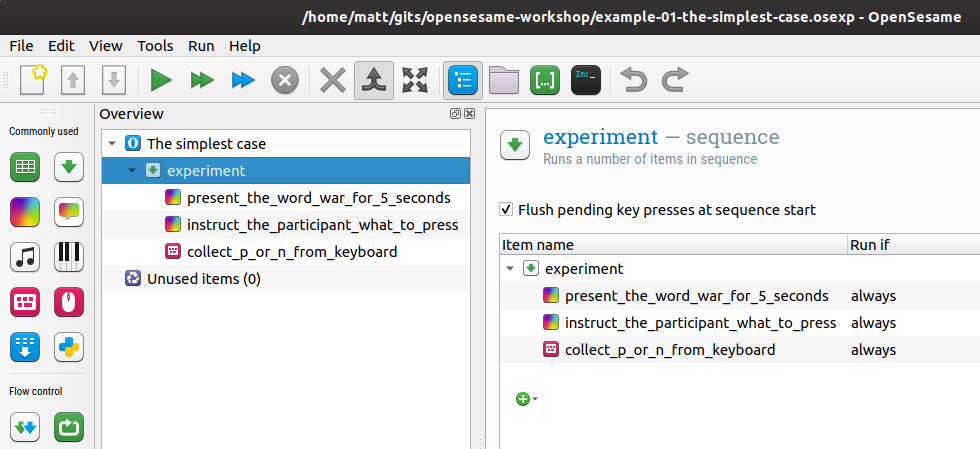
\includegraphics[width=\textwidth]{screenshots/example-01.png}
\caption{example 01 screenshot}
\label{example-01-png}
\end{figure}

Even in this very simple experiment, we can learn a lot about the way OpenSesame works by going through the exercises below.

\begin{enumerate}
\item The first thing for you to do is to run the experiment. In OpenSesame there are several different ways to run an experiment. In the top-left of the interface there are three buttons with arrows facing right -- each one runs the experiment in a different way, as described next:

\begin{enumerate}
\item The big green single arrow is what you use to run an experiment while you are collecting real data with a real participant. In this mode, the experiment will ask you for a participant number, and the filename for the results file; it will run full-screen; and it will write out a results file at the end. While you are still developing the experiment, like we are now, you should use one of the double-arrows: 
\item The green double-arrow does the same as the single green arrow, except that instead of running full-screen, it runs in a window about half the size of the screen. This is handy because if there is an error, you will have a better chance of seeing why it went wrong.
\item The blue double-arrow also runs in a smaller window, but it differs in that it doesn't prompt you for a participant number, and doesn't write a results file. The blue double-arrow is a sort of "quick-run" option. 
\end{enumerate}

Use the blue double-arrow to run the experiment now. %
\marginnote{\textsc{Excercise 1: Test-run the experiment}}%
You are aiming to verify that the experiment runs without throwing any errors; and to check that it does what you expect: i.e., it should show the word "war" for 5 seconds; then tell you what the response options are; and then wait for you to press either "p" or "n", but refuse to proceed if you press some other key.

\item The next thing is to explore the experiment to find out how each of the three parts of the flow works. When you click on an item in the \emph{list-view} (or \emph{flow-chart} if you prefer that term) on the left hand side of the interface, the right-hand-side will show a detailed view of what that item does, and what options you can set for that item. %
\marginnote{\textsc{Excercise 2: Explore the experiment}}%
You are aiming to answer the following questions:
\begin{enumerate}
\item How do we specify that "war" is the text that gets displayed?
\item How do we specify that "war" should be displayed for 5 seconds (rather than some other duration)?
\item How do we make sure that the experiment will not accept any keyboard responses other than "p" or "n"?
\item How do we make the experiment wait for as long as it takes the participant to respond, instead of timing out after some fixed interval of time?
\end{enumerate}
\end{enumerate}

\section{More realistic cases: multiple trials using sequences and loops}
\subsection{sequencing}
\subsection{looping}

\section{Stimulus types available}

\section{Response types available}

\section{Feedback to participants}

\section{Eye-tracking (on any tracker)}

\section{Counterbalancing, and other uses of python)}

\section{Cross-platform support}

\section{Some comparisons of OpenSesame against alternative software}

%\bibliography{handout}

\end{document}

